\section{Resultados}
\label{resultados}

En esta sección hablaremos de los resultados obenidos por las implementaciones de los algoritmos vistos.

\subsection{Exploración de resultados con error num´erico}

El error numérico en la resolución de sistemas de ecuaciones lineales mediante eliminación gaussiana impacta en la estabilidad y precisión de las soluciones obtenidas. Considerando matrices con diferentes números de condición buscamos medir el error entre las soluciones teóricas y las obtenidas por el algoritmo, utilizando representaciones de punto flotante de 32 y 64 bits. A través de la variación de un parámetro $\epsilon$, se exploran los efectos de la estabilidad numérica sobre las soluciones, evaluando cómo la precisión disminuye a medida que $\epsilon$ se reduce, y cómo el número de bits afecta el error final.

Se tiene el sistema de ecuaciones lineales con A y b igual a:

\[ \begin{bmatrix}
1 & 2+\epsilon & 3-\epsilon\\
1-\epsilon & 2 & 3+\epsilon\\
1+\epsilon & 2-\epsilon & 3
\end{bmatrix} ,
\begin{bmatrix}
6\\
6\\
6
\end{bmatrix}\]

Se calcula la matriz inversa de A, $A^{-1}$:
\begin{center}
$\begin{bmatrix}
\frac{\epsilon+1}{18\epsilon} & \frac{\epsilon-8}{18\epsilon} & \frac{\epsilon+7}{18\epsilon}\\
\frac{\epsilon+7}{18\epsilon} & \frac{\epsilon-2}{18\epsilon} & \frac{\epsilon-5}{18\epsilon}\\
\frac{\epsilon-5}{18\epsilon} & \frac{\epsilon+4}{18\epsilon} & \frac{\epsilon+1}{18\epsilon}
\end{bmatrix}$
\end{center}

Con este resultado es sencillo notar que el único $\epsilon$ que genera que A no tenga inversa es 0. Para el resto, A tiene inversa y por lo tanto el sistema de ecuaciones tiene una única solución. Cuando multiplicamos a $A^{-1}$ por b, obtenemos que el vector solución es x$^t$ = [1, 1, 1], independientemente del $\epsilon$. Por lo tanto, la solución del algoritmo de pivoteo parcial debería devolver siempre x$^t$ = [1, 1, 1]. Sin embargo, se espera que por error numérico esto no sea así. 

La norma infinito de $A$ es 6 y la de $A^{-1}$ es $\frac{\epsilon+16}{18\epsilon}$. Por lo tanto el numero de condición para $A$ es $\frac{\epsilon+16}{3\epsilon}$. Si $\epsilon$ tiende a cero, el numero de condición para $A$ es infinito. Si en cambio, tiende a infinito, el numero de condición es 1/3. Entonces, cuanto más grande es $\epsilon$, más chico es el numero de condición y más estable es A. 

El gráfico a continuación muestra la comparación entre el error absoluto vs $\epsilon$ para variables de 32 bits y 64 bits:

\begin{figure}[htbp]
\centerline{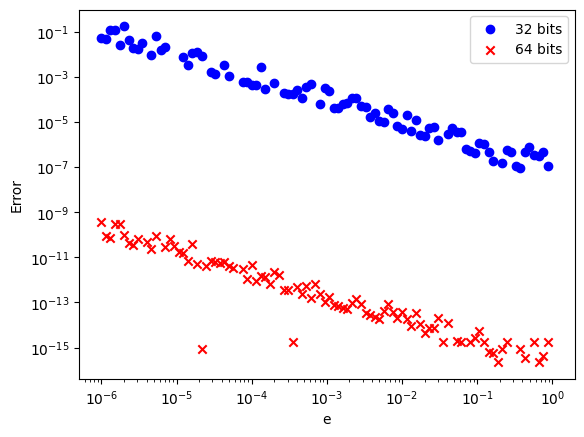
\includegraphics[scale=0.50]{./img/error_numerico_32vs64.png}}
\caption{Error Numérico}
\label{result_errorNumerico}
\end{figure}

Como podemos observar, el error numérico se encuentra delimitado con tope inferior y superior para cada $\epsilon$ y a menores $\epsilon$ el error numérico en la solución es mas grande y decrece a medida que aumenta $\epsilon$. De la misma forma, el error numérico para 64 bits es varios ordenes de magnitud más chico que para 32 bits, ya que se aumenta la precisión en los cálculos.



\subsection{Verificación de la implementación}
Para probar nuestra implementación de sistema tridiagonal se nos pidió resolver una serie de ecuaciones diferenciales. Debemos encontrar \textit{u} para el problema $\frac{\partial^2}{\partial x^2}u = d$ utilizando la matriz tridiagonal del operador laplaciano.
Como mencionamos anteriormente (sección \ref{Intro_laplaciano}), para el caso unidimensional la operación discreta de $\frac{\partial^2}{\partial x^2}u = d$ está dada por:

u$_{i-1}$ - 2u$_{i}$ + u$_{i+1}$ = d$_{i}$

Esta ecuación forma un sistema matricial como se muestra en la figura \ref{laplaciano}. Esta matriz es tridiagonal y siguiendo la estructura de la matriz de la sección \ref{tridiagonal} toma valores:

\begin{itemize}
    \item a: vector de valores 1.
    \item b: vector de valores -2.
    \item c: vector de valores 1.
\end{itemize}

\begin{figure}[H]
    \[ \begin{bmatrix}
-2 & 1 & & & 0\\
1 & -2 & 1 & & & \\
    & 1 & -2 & \ddots & \\
    &    & \ddots &  \ddots & 1\\
0   &    &   & 1 & -2
     \end{bmatrix}
     \begin{bmatrix}
           u_{1}\\
           u_{2} \\
           u_{3}\\ 
           \vdots\\ 
           u_{n}  
     \end{bmatrix}
      =
     \begin{bmatrix}
          d_{1} \\
          d_{2}\\
          d_{3}\\
         \vdots\\ 
         d_{n}  
     \end{bmatrix} \]
     \caption{Forma matricial}\label{laplaciano}
\end{figure}
Por esta estructura,  el algoritmo de eliminación gaussiana para tridiagonales puede aplicarse eficientemente resolviendo el sistema de ecuaciones resultantes de la discretización. Además, como la matriz es diagonal dominante, no es necesario el pivoteo pues no hay riesgo de división por cero. 

De esta forma, se modelaron los tres vectores $d$ a los cuales nombramos como d$\_vect\_a$, d$\_vec\_b$  y d$\_vec\_c$, que representan las ecuaciones requeridas que se pueden ver a continuación con parámetro $n=101$  y se calcularon las segundas derivadas para los tres casos utilizando el algoritmo que se encuentra en la sección \ref{tridiagonal}.

\begin{enumerate}[label=\alph*)] % (a), (b), (c), ...
\label{ec_ej4}
\item d$_{i}$ = 
    $\begin{cases}
      0\\
      \frac{4}{n} & i=\lfloor \frac{n}{2} \rfloor   +1
    \end{cases}$

\item d$_{i}$ = $\frac{4}{n^{2}}$

\item d$_{i}$ = $\frac{-1+2i}{(n-1)}\frac{12}{n^{2}}$

\end{enumerate}


Con estos resultados, se creó un único gráfico que se muestra en la siguiente Figura \ref{result_laplaciano} obteniendo el resultado esperado.

\begin{figure}[H]
\centerline{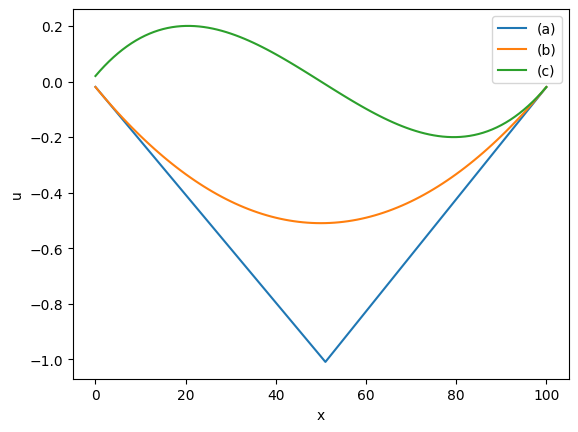
\includegraphics[scale=0.45]{./img/resultado_tridiag}}
\caption{Resultado de las funciones}
\label{result_laplaciano}
\end{figure}

Analizando con mayor profundidad cada función:\par
\begin{enumerate}
    \item[a)] La derivada segunda de la función (a) es 0 para todo x distinto a $i = n/2 + 1$. Luego, la derivada primera de la función (a) es constante para todo x $\not =$ i,lo que implica que la función es lineal para todo x $\not =$ i. Por lo que i es un punto de inflexión. Como la derivada segunda en i es positiva, la función tiene que ser cóncava para los positivos. Esta función descripta es coherente con la figura graficada.

    \item[b)] La derivada segunda de la función (b) es $\frac{4}{n^2}$ para todo x. Entonces, la derivada primera es lineal para todo x, lo que implica que la función es cuadrática para todo x. La función graficada se corresponde con una cuadrática.

    \item[c)] La derivada segunda de la función (c) es una función lineal para todo x. Esto significa que la derivada primera es cuadrática, implicando que la función debe ser un polinomio de grado tres (cúbica). La función graficada se corresponde con una cúbica.
\end{enumerate}



\subsection{Tiempos de cómputo}
Como explicamos anteriormente, los diferentes algoritmos tienen complejidades computacionales muy distintas, lo que afecta significativamente el tiempo de ejecución y los recursos necesarios para resolver un problema.

En el caso de la eliminación gaussiana, el algoritmo con pivoteo tiene una complejidad cúbica ($\mathcal{O}$(n$^3$)), lo que significa que el tiempo de ejecución crece rápidamente a medida que aumenta el tamaño de la matriz. Por otro lado, los algoritmos diseñados específicamente para matrices con estructura especial, como el caso de las matrices tridiagonales, pueden reducir esa complejidad a $\mathcal{O}$(n), lo que implica una mejora considerable en términos de rendimiento.Por lo tanto, Lo esperado es que el algoritmo tridiagonal sea notablemente más rápido a comparación del algoritmo de eliminación gaussiana con pivoteo

Para evaluar el rendimiento de los distintos algoritmos de eliminación gaussiana, se generaron matrices y vectores correspondientes a cada tamaño seleccionado. Posteriormente, se implementaron los algoritmos de eliminación gaussiana con pivoteo, eliminación gaussiana para matrices tridiagonales, tanto en su versión estándar como en la versión con precomputo, para dimensiones que corresponden a potencias de dos (2$^k$). Este proceso fue repetido 10 veces, registrando el tiempo mínimo de ejecución en cada iteración. Esta repetición busca mitigar el posible efecto de las variaciones causadas por la organización del computador (posición de las variables en memoria por ejemplo).

Considerando, las complejidades temporales teóricas de los algoritmos:

\begin{itemize}
    \item Eliminación Gaussiana con pivoteo: $O(n^{3})$
    \item Eliminación Gaussiana para matrices tridiagonales estándar: $O(n)$
    \item Eliminación Gaussiana para matrices tridiagonales con precomputo: $O(n)$
\end{itemize}


Definimos \textit{A} como la matriz Laplaciana, es decir, aquella matriz que tiene a -2 como elementos de la diagonal y a 1 como los elementos de las dos subdiagonales. Obtenemos el siguiente resultado (figura \ref{result_ej5})

\begin{figure}[H]
\centerline{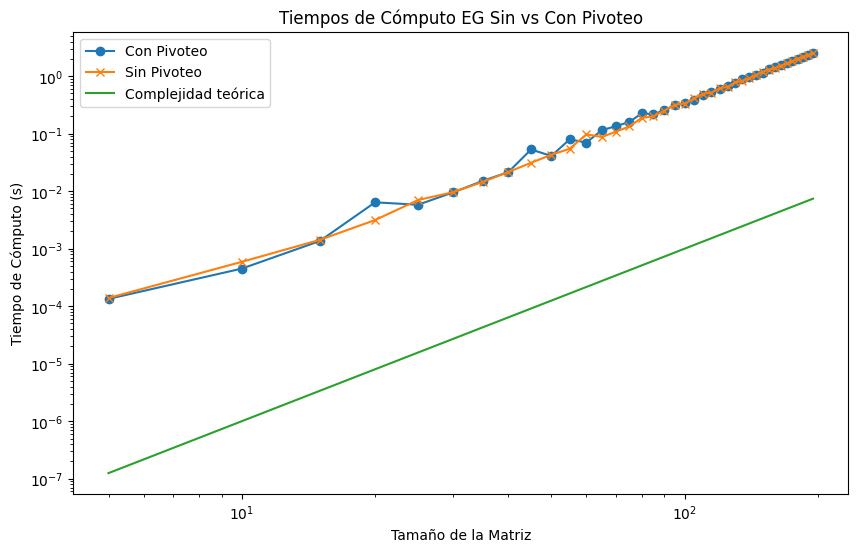
\includegraphics[scale=0.45]{./img/tiempos_EGsinVsConPivoteo.png}}
\caption{Tiempo de computo para EG con pivoteo y EG en un sistema tridiagonal}
\label{result_ej5}
\end{figure}

Como era esperado, como los algoritmos de las matrices tridiagonales trabajan a nivel vectorial, modificando los valores de los vectores b y c, la complejidad temporal mejora.

Por otro lado, realizamos la comparación entre la implementación de EG para un sistema tridiagonal y su variante con precómputo. En la figura \ref{result_ej5_2do} podemos observar claramente el beneficio en el tiempo de ejecución al utilizar la segunda variante del algoritmo, especialmente cuando la cantidad de sistemas a resolver es crecientemente superior a la dimensión del sistema.

\begin{figure}[H]
\centerline{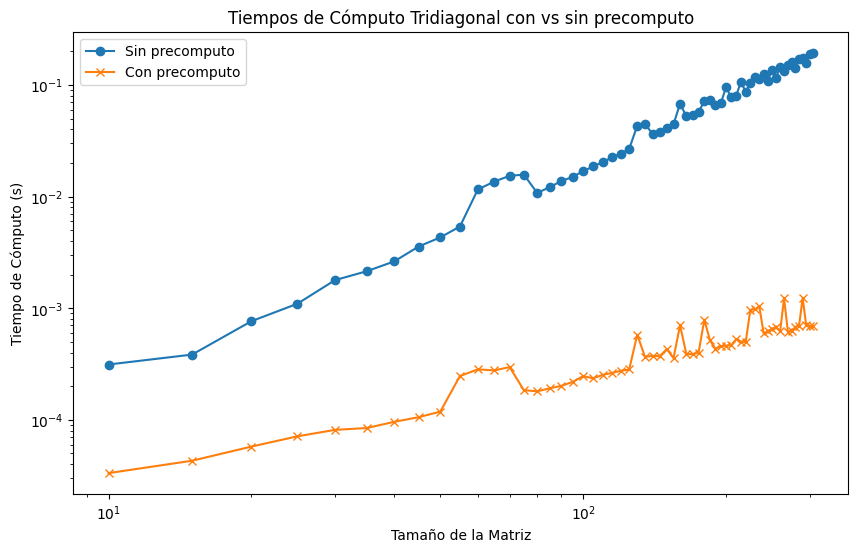
\includegraphics[scale=0.45]{./img/tiempos_tridiagConVsSinP.png}}
\caption{Tiempo de computo para Eliminación Gaussiana tridiagonal estandar vs. precomputada}
\label{result_ej5_2do}
\end{figure}

%Los resultados obtenidos se pueden ver en la sección \ref{resultados}


\subsection{Simulación de difusión}

Para expresar la ecuación de difusión se considera el incremento para el paso \textit{k}, $u^k - u^{k-1}$ como una
fracción ($\alpha$) del operador laplaciano aplicado a $u^{k-1}$ (ecuación explícita) y a $u^{k}$ (ecuación implícita):
\begin{center}
  $u_i^{(k)} - u_i^{(k-1)}$ = $\alpha(u_{i-1}^{(k-1)} - 2u_i^{(k-1)} + u_{i+1}^{(k-1)}) - Eq (3)$
\end{center}

\begin{center}
  $u_i^{(k)} - u_i^{(k-1)}$ = $\alpha(u_{i-1}^{(k)} - 2u_i^{(k)} + u_{i+1}^{(k)}) - Eq (4)$
\end{center}

Reordenando los términos, obtenemos una solución de forma explícita para la ecuación (3). Ésta responde a la forma $u^{(k)} = A \times u^{(k-1)}$. Por otro lado, reordenando los términos de la ecuación (4) obtenemos una solución de forma implícita: A$\times u^{(k)}$ = $u^{(k-1)}$. De esta forma, para obtener la evolución, resolvemos el sistema de ecuaciones para cada paso $k$.

Dada la ecuación:

\begin{equation}
u_{i}^{(k)} - u_{i}^{(k-1)} = \alpha \times (u_{i-1}^{(k)} - 2u_{i}^{(k)} + u_{i+1}^{(k)})
\end{equation}

Se observa que la siguiente ecuación es la ecuación anterior expresada en forma matricial:

\begin{equation}
(I - \alpha \times H) \times u^{(k)} = u^{(k-1)}
\end{equation}

donde:

\begin{itemize}
  \item u$^{(j)}$: vector u en el paso j de difusión
  \item H: matriz Laplaciana de n $\times$ n
  \item I: matriz Identidad de n $\times$ n
\end{itemize}

Demostración:

\begin{equation}
u_{i}^{(k)} - u_{i}^{(k-1)} = \alpha \times (u_{i-1}^{(k)} - 2u_{i}^{(k)} + u_{i+1}^{(k)}) \space \forall i \in [1, n]
\end{equation}

\begin{equation}
\begin{bmatrix}
u_{1}\\
...\\
u_{n}
\end{bmatrix}^{(k)}
-
\begin{bmatrix}
u_{1}\\
...\\
u_{n}
\end{bmatrix}^{(k-1)}
=
\alpha \times H \times
\begin{bmatrix}
u_{1}\\
...\\
u_{n}
\end{bmatrix}^{(k)}
\end{equation}

\begin{equation}
u^{(k)} - u^{(k-1)} = \alpha \times H \times u^{(k)}
\end{equation}

\begin{equation}
u^{(k)} - \alpha \times H \times u^{(k)} =  u^{(k-1)}
\end{equation}

\begin{equation}
(I - \alpha H) \times u^{(k)} = A \times u^{(k)} =  u^{(k-1)}
\end{equation}

Consecuentemente, A = I - $\alpha \times$ H.


Utilizando la última formulación, logramos generar soluciones estables para todos los valores.

Para la solución implícita podemos notar que se genera un sistema tridiagonal, lo que nos permite utilizar el algoritmo de eliminación Gaussiana para sistemas tridiagonales. La eliminación Gaussiana no requiere pivoteo por la estructura de la matriz de derivada segunda. La triangulación finaliza en una matriz donde los elementos de la diagonal principal son: $a_{ii} = - \frac{i+1}{i}$. 
Es así que, como en ningún paso queda un elemento de la diagonal igual a cero, no se requiere pivoteo.\par

Para investigar los distintos grados de difusión utilizamos lso parámetros n = 101, r = 10, m = 1000 y ajustamos el parámetro $\alpha$, el cual se considera como una medida de la tasa de difusión en un modelo específico. Este valor representa una fracción del operador laplaciano, el cual interviene directamente en el cálculo de la difusión de un paso discreto al siguiente.
Al modificar $\alpha$, se observa cómo varía el patrón y la velocidad de difusión de la entidad en cuestión. Por ejemplo, la primer experimentación que se realizo se tomó $\alpha$ = 1 obteniendo el resultado que se muestra en la figura \ref{fig:alpha_1}. Se pudo observar que el gráfico obtenido es equivalente al brindado por la cátedra.

A partir de esto, se planteo que a partir de valores más altos de $\alpha$, la difusión sería mayor, siendo probable que veamos una difusión más rápida, donde la entidad se propaga más lejos desde su punto de origen en un período de tiempo determinado.
Mientras que con valores más bajos de $\alpha$, la difusión sería menor siendo probable que la difusión sea más lenta y limitada en alcance.
Para realizar al experimentación, se crearon los vectores con los mismos datos para $\alpha$ = 1, variando únicamente este ultimo parámetro al cual se le asigno valores de 0.1, 0.5 y 2.
A continuación, se generaron los cuatro gráficos que se pueden observar en las figuras \ref{fig:awesome_image1}, \ref{dif0.5} y \ref{fig:result_dif}.
%\begin{figure}[htbp]
%\centerline{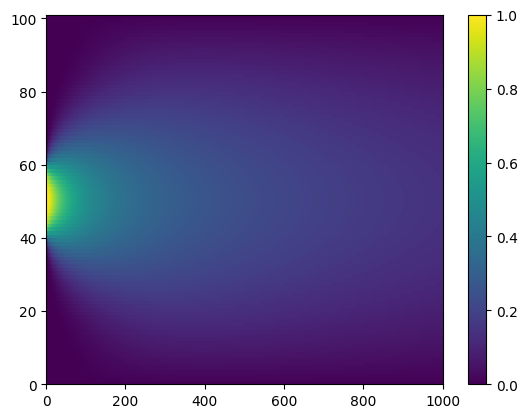
\includegraphics[scale=0.45]{./img/result_dif.png}}
%\caption{Resultado difusión para $\alpha$ = 1}
%\label{result_dif}
%\end{figure}

\begin{figure}[H] 
  \label{ fig7} 
  \begin{minipage}[b]{0.5\linewidth}
    \centering
    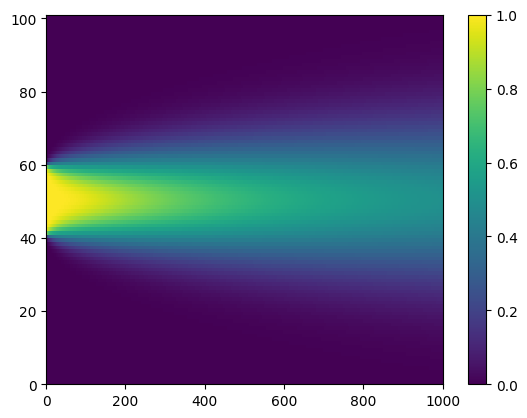
\includegraphics[width=.5\linewidth]{./img/alfa1.png}
  \caption{Difusión $\alpha$ = 0.1}\label{fig:awesome_image1} 
    \vspace{4ex}
  \end{minipage}%%
  \begin{minipage}[b]{0.5\linewidth}
      \centering
    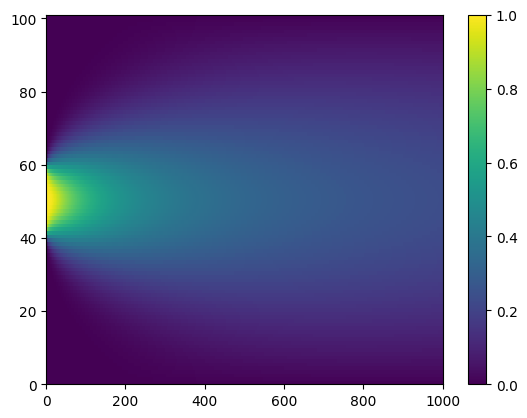
\includegraphics[width=.5\linewidth]{./img/alfa05.png} 
    \caption{Difusión $\alpha$ = 0.5} \label{dif0.5} 
    \vspace{4ex}
  \end{minipage} 
  \begin{minipage}[b]{0.5\linewidth}
    \centering
    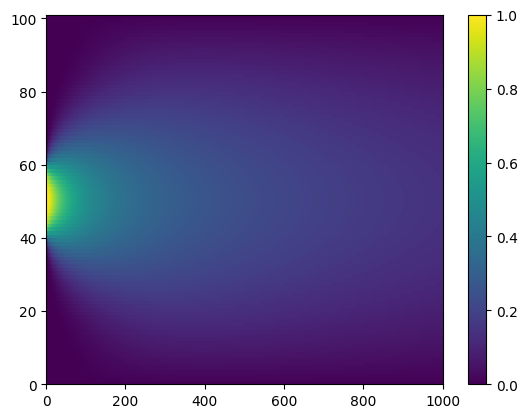
\includegraphics[width=.5\linewidth]{./img/result_dif.png}
  \caption{Difusion $\alpha$ = 1}\label{fig:alpha_1}
    \vspace{4ex}
  \end{minipage}%% 
  \begin{minipage}[b]{0.5\linewidth}
    \centering
    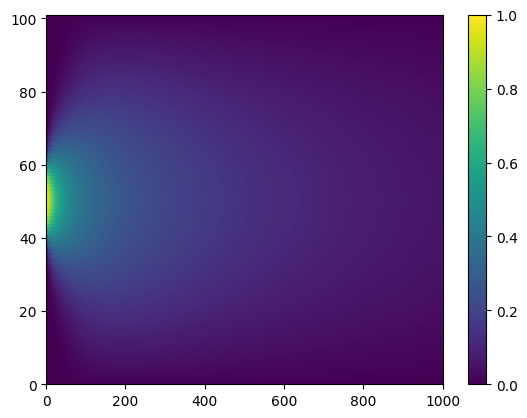
\includegraphics[width=.5\linewidth]{./img/alfa2.png}
  \caption{Difusión $\alpha$ = 2}\label{fig:result_dif}
    \vspace{4ex}
  \end{minipage} 
\end{figure}








\subsubsection{Simulación de difusión 2D}

Al implementar la simulación de la difusión de calor en una placa de 15x15 unidades, se considera una fuente de calor en el punto central con una temperatura constante de 100 unidades, mientras que los bordes de la placa permanecen a 0 en todo momento. Esta simulación, basada en el método implícito, se rige por la ecuación de difusión, que modela cómo el calor se propaga a lo largo del tiempo.
 Como utilizaremos el método implícito, cada paso de tiempo requiere resolver un sistema de ecuaciones lineales. Esto nos garantiza estabilidad, incluso si el coeficiente de difusión $\alpha$ = 0.1 varía.
Por otro lado, a diferencia de la simulación anterior la matriz resultante en 2D no será tridiagonal, sino pentadiagonal, debido a que cada punto de la placa interactúa con sus vecinos en las cuatro direcciones.
En la figura \ref{result_dif} podemos visualizar cómo cambia la distribución de temperatura en la placa a medida que pasa el tiempo.

\begin{figure}[H]
\centerline{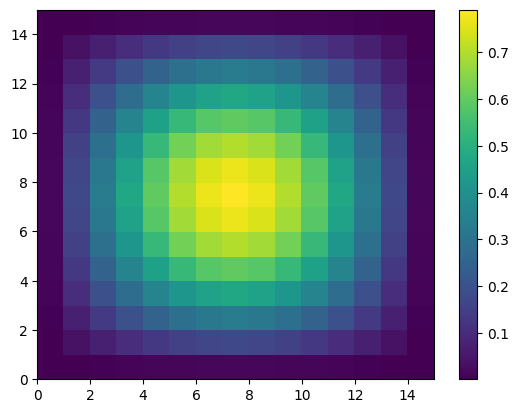
\includegraphics[scale=0.45]{./img/2Dcasoborde0.png}}
\caption{Resultado simulación de difusión de calor en una placa 2D, condiciones de borde con temperatura 0}
\label{result_dif}
\end{figure}



Realizando la comparación de los tiempos de cómputo para la resolución del sistema de ecuaciones de difusión de calor en 2D utilizando los métodos vistos anteriormente (eliminación gaussiana con y sin pivoteo) pudimos observar en la figura \ref{tiempos_dif2D} que, como era de esperar, el tiempo de cómputo aumenta de manera rápida a medida que el tamaño de la matriz crece. Esto se relaciona con el número de operaciones realizadas para resolver el sist. de ec. lineales ya que ésta crece aproximadamente de manera cúbica con el tamaño de la matriz.
Para matrices pequeñas (hasta tamaño 10x10), el tiempo de cómputo es prácticamente el mismo por lo que sugiere que el pivote no añade un costo computacional significativo. Sin embargo, para matrices más grandes (12x12 en adelante), se empieza a notar una diferencia pues el pivoteo mejora la estabilidad numérica del sistema.

\begin{figure}[H]
\centerline{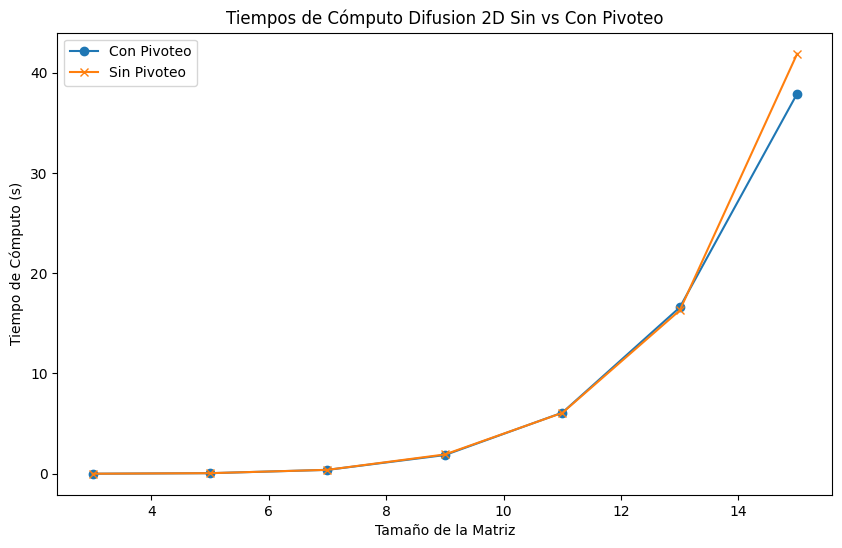
\includegraphics[scale=0.45]{./img/Dif2D_tiempos.png}}
\caption{ Tiempos de cómputo para la resolución del sistema de ecuaciones de difusión de calor en 2D}
\label{tiempos_dif2D}
\end{figure}



Dado que los bordes tienen una temperatura fija de 0, el calor tenderá a disiparse hacia estos, lo que limitará su propagación.
Podemos observar que en el instante t=10 en la figura \ref{instante10}, el calor ya comenzó a propagarse significativamente desde el centro, pero todavía no ha llegado a los bordes de la placa, lo que es esperable porque aún estamos en un tiempo relativamente temprano en la simulación. A su vez, la distribución suave de la temperatura en los alrededores de la fuente central sugiere que el método implícito utilizado está funcionando bien, ya que evita oscilaciones o comportamientos inestables.



\begin{figure}[H] 
  \label{ fig7} 
  \begin{minipage}[b]{0.5\linewidth}
    \centering
    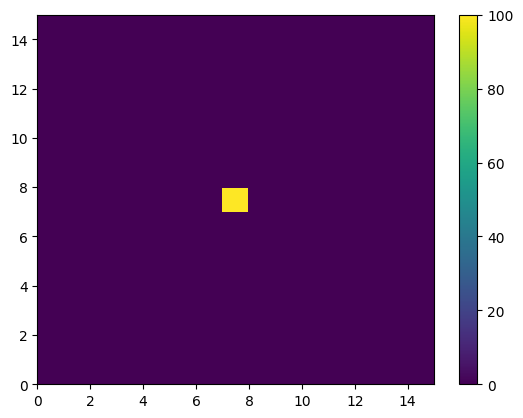
\includegraphics[width=.5\linewidth]{./img/instante_0.png}
  \caption{Instante $t$ = 0}\label{instante0} 
    \vspace{4ex}
  \end{minipage}%%
  \begin{minipage}[b]{0.5\linewidth}
      \centering
    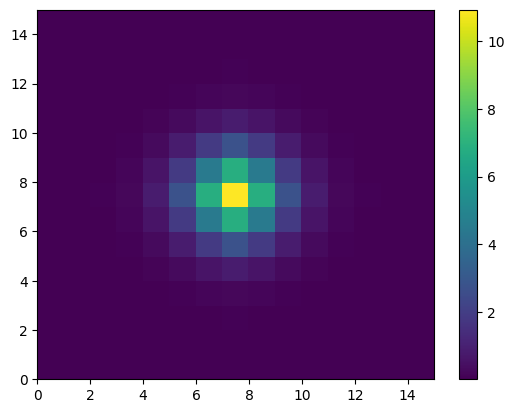
\includegraphics[width=.5\linewidth]{./img/instante_10.png} 
    \caption{Instante $t$ = 10} \label{instante10} 
    \vspace{4ex}
  \end{minipage} 
  \begin{minipage}[b]{0.5\linewidth}
    \centering
    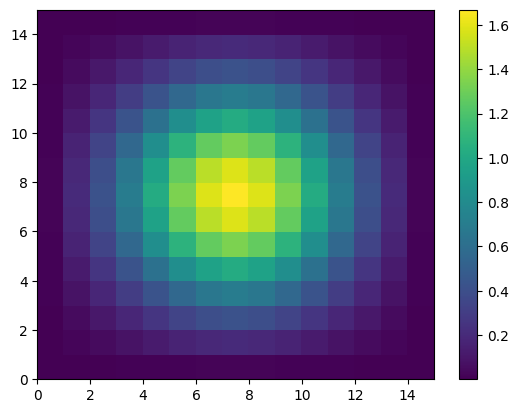
\includegraphics[width=.5\linewidth]{./img/instante_50.png}
  \caption{Instante $t$ = 50}\label{instante50}
    \vspace{4ex}
  \end{minipage}%% 
  \begin{minipage}[b]{0.5\linewidth}
    \centering
    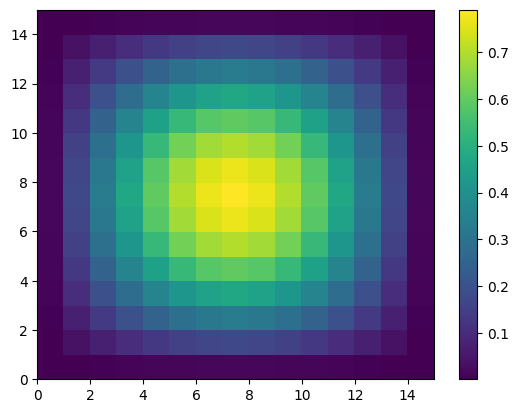
\includegraphics[width=.5\linewidth]{./img/instante_100.png}
  \caption{Instante $t$ = 100}\label{instante100}
    \vspace{4ex}
  \end{minipage} 
\end{figure}






\iffalse
    \subsection{Resultado de eliminación Gaussiana sin pivoteo}
    \label{resultados EG}

    \subsubsection{Ejercicio 1.1}
    El pseudocódigo de la función implementada se puede encontrar en la sección \ref{EG_sinP}

    \subsubsection{Ejercicio 1.2}

    Ya est´á dentro de la introducci´ón.



    Si tomamos de ejemplo a la siguiente matriz:

    \begin{center}
    $\begin{bmatrix}
    0 & 1 & -1 & 3\\
    -2 & -0.5 & 0 & 0\\
    4 & 1 & -2 & 4\\
    -6 & -1 & 2 & -3
    \end{bmatrix}$
    \end{center}
                  
    Es esperado que al procesarla se produzca un error debido a que para resolver el sistema necesitamos intercambiar filas y columnas para llevar la matriz a una forma triangular superior y el algoritmo no lo realiza, pues solo se permite operaciones de multiplicación y suma para reducir los elementos debajo de la diagonal principal.

    \subsection{Resultado de eliminación Gaussiana con pivoteo}
    \label{resultados EG c/p}
    \subsubsection{Ejercicio 2.1}
    El pseudocódigo de la función implementada se puede encontrar en la sección \ref{seccion_EG_pivot}

    \subsubsection{Ejercicio 2.2}

Movido a la introducción

\fi




\iffalse
    \subsection{Ejercicio 2.3}

    Se tiene el sistema de ecuaciones lineales con A y b igual a:

    \[ \begin{bmatrix}  
    1 & 2+\epsilon & 3-\epsilon\\
    1-\epsilon & 2 & 3+\epsilon\\
    1+\epsilon & 2-\epsilon & 3
    \end{bmatrix} ,
    \begin{bmatrix}
    6\\
    6\\
    6
    \end{bmatrix}\]
    
    Se calcula la matriz inversa de A, $A^{-1}$:    
    \begin{center}
    $\begin{bmatrix}
    \frac{\epsilon+1}{18\epsilon} & \frac{\epsilon-8}{18\epsilon} & \frac{\epsilon+7}{18\epsilon}\\
    \frac{\epsilon+7}{18\epsilon} & \frac{\epsilon-2}{18\epsilon} & \frac{\epsilon-5}{18\epsilon}\\
    \frac{\epsilon-5}{18\epsilon} & \frac{\epsilon+4}{18\epsilon} & \frac{\epsilon+1}{18\epsilon}
    \end{bmatrix}$
    \end{center}

    Con este resultado es sencillo notar que el único $\epsilon$ que genera que A no tenga inversa es 0. Para el resto, A tiene inversa y por lo tanto el sistema de ecuaciones tiene una única solución. Cuando multiplicamos a $A^{-1}$ por b, obtenemos que el vector solución es x$^t$ = [1, 1, 1], independientemente del $\epsilon$. Por lo tanto, la solución del algoritmo de pivoteo parcial debería devolver siempre x$^t$ = [1, 1, 1]. Sin embargo, se espera que por error numérico esto no sea así. 

    La norma infinito de $A$ es 6 y la de $A^{-1}$ es $\frac{\epsilon+16}{18\epsilon}$. Por lo tanto el numero de condición para $A$ es $\frac{\epsilon+16}{3\epsilon}$. Si $\epsilon$ tiende a cero, el numero de condición para $A$ es infinito. Si en cambio, tiende a infinito, el numero de condición es 1/3. Entonces, cuanto más grande es $\epsilon$, más chico es el numero de condición y más estable es A. 

    El gráfico a continuación muestra la comparación entre el error absoluto vs $\epsilon$ para variables de 32 bits y 64 bits:

    \begin{figure}[htbp]
    \centerline{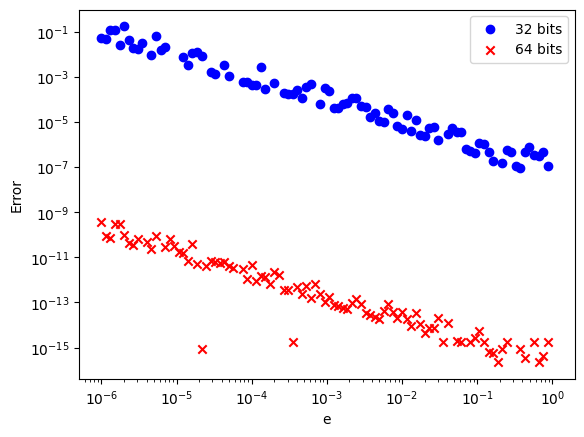
\includegraphics[scale=0.50]{./img/error_numerico_32vs64.png}}
    \caption{Error Numérico}
    \label{result_errorNumerico}
    \end{figure}

    Como podemos observar, el error numérico se encuentra delimitado con tope inferior y superior para cada $\epsilon$ y a menores $\epsilon$ el error numérico en la solución es mas grande y decrece a medida que aumenta $\epsilon$. De la misma forma, el error numérico para 64 bits es varios ordenes de magnitud más chico que para 32 bits, ya que se aumenta la precisión en los cálculos.

\fi


%%%%%%%%%%%%%%%%%%%%%%%%%%%%%%
\iffalse
    \subsection{Resultado Verificación de la implementación}
    \label{resultados derivada}
    Realizamos el cálculo de la derivada segunda de manera discreta para las tres funciones especificadas por la cátedra utilizando la implementación de eliminación Gaussiana para un sistema tridiagonal.
    Se generaron los vectores d$\_vect\_a$, d$\_vec\_b$  y d$\_vec\_c$ que representan las funciones que se encuentran en la sección \ref{tridiagonal} y se calcularon las segundas derivadas para los tres casos.
    Con estos resultados, se creó un único gráfico que se muestra en la siguiente Figura \ref{result_laplaciano} obteniendo el resultado esperado.

    \begin{figure}[H]
    \centerline{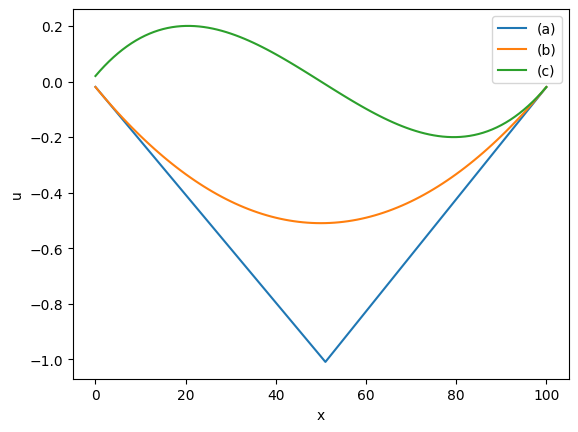
\includegraphics[scale=0.45]{./img/resultado_tridiag}}
    \caption{Resultado de las funciones}
    \label{result_laplaciano}
    \end{figure}

    Analizando con mayor profundidad cada función:\par
    \begin{enumerate}
        \item[a)] La derivada segunda de la función (a) es 0 para todo x distinto a $i = n/2 + 1$. Luego, la derivada primera de la función (a) es constante para todo x $\not =$ i,lo que implica que la función es lineal para todo x $\not =$ i. Por lo que i es un punto de inflexión. Como la derivada segunda en i es positiva, la función tiene que ser cóncava para los positivos. Esta función descripta es coherente con la figura graficada.

        \item[b)] La derivada segunda de la función (b) es $\frac{4}{n^2}$ para todo x. Entonces, la derivada primera es lineal para todo x, lo que implica que la función es cuadrática para todo x. La función graficada se corresponde con una cuadrática.

      \item[c)] La derivada segunda de la función (c) es una función lineal para todo x. Esto significa que la derivada primera es cuadrática, implicando que la función debe ser un polinomio de grado tres (cúbica). La función graficada se corresponde con una cúbica.
    \end{enumerate}
\fi    
    
%%%%%%%%%%%%%%%%%%%%%%%%%%%%%%
    
    

\iffalse
    \subsection{Resultado Tiempos de cómputo}
    \label{resultados tiempo}
    \subsubsection{Ejercicio 5.1}
    El objetivo de este ejercicio es obtener de forma experimental la complejidad temporal de los algoritmos utilizados en los puntos anteriores: eliminación Gaussiana con pivoteo, eliminación Gaussiana para matrices tridiagonales estándar y con precomputo. Las complejidades temporales teóricas de los algoritmos son:

    \begin{itemize}
        \item Eliminación Gaussiana con pivoteo: $O(n^{3})$
        \item Eliminación Gaussiana para matrices tridiagonales estándar: $O(n)$
        \item Eliminación Gaussiana para matrices tridiagonales con precomputo: $O(n)$
    \end{itemize}

    El algoritmo de Eliminación Gaussiana con pivoteo tiene un triple for, necesario para la triangulación de la matriz A. Lo que genera que la complejidad temporal sea cúbica. En cambio los algoritmos de las matrices tridiagonales trabajan a nivel vectorial, modificando los valores de los vectores b y c. Lo que genera que la complejidad temporal sea lineal.

    Para este ejercicio se definió \textit{A} como la matriz Laplaciana, es decir, aquella matriz que tiene a -2 como elementos de la diagonal y a 1 como los elementos de las dos subdiagonales.

    \begin{figure}[H]
    \centerline{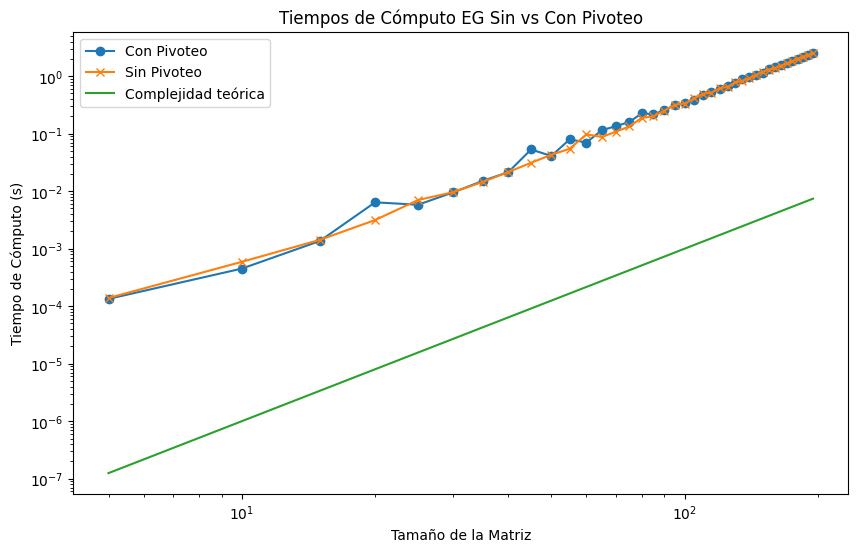
\includegraphics[scale=0.45]{./img/tiempos_EGsinVsConPivoteo.png}}
    \caption{Tiempo de computo para EG con pivoteo y EG en un sistema tridiagonal}
    \label{result_ej5}
    \end{figure}
\fi

%%%%%%%%%%%%%%%%%%%%%%%%%%%%%%

\iffalse
    \subsubsection{Ejercicio 5.2}

    Con el resultado obtenido, se ve claramente el beneficio en el tiempo de ejecución al utilizar la segunda variante del algoritmo, especialmente cuando la cantidad de sistemas a resolver es crecientemente superior a la dimensión del sistema.

    \begin{figure}[H]
    \centerline{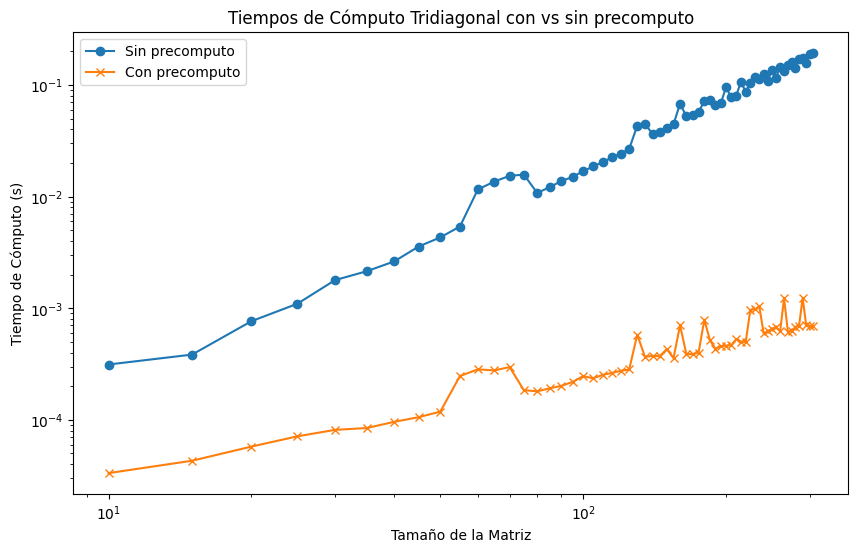
\includegraphics[scale=0.45]{./img/tiempos_tridiagConVsSinP.png}}
    \caption{Tiempo de computo para Eliminación Gaussiana tridiagonal estandar vs. precomputada}
    \label{result_ej5_2do}
    \end{figure}

\fi

%%%%%%%%%%%%%%%%%%%%%%%%%%%%%%
\iffalse
    \subsection{Resultado Difusión}
    \label{difusion}
    \subsubsection{Ejercicio 6.1}
    Dada la ecuación:
    
    \begin{equation}
    u_{i}^{(k)} - u_{i}^{(k-1)} = \alpha \times (u_{i-1}^{(k)} - 2u_{i}^{(k)} + u_{i+1}^{(k)})
    \end{equation}

    Se observa que la siguiente ecuación es la ecuación anterior expresada en forma matricial:

    \begin{equation}
    (I - \alpha \times H) \times u^{(k)} = u^{(k-1)}
    \end{equation}

    donde:

    \begin{itemize}
      \item u$^{(j)}$: vector u en el paso j de difusión
      \item H: matriz Laplaciana de n $\times$ n
      \item I: matriz Identidad de n $\times$ n
    \end{itemize}

    Demostración:

    \begin{equation}
    u_{i}^{(k)} - u_{i}^{(k-1)} = \alpha \times (u_{i-1}^{(k)} - 2u_{i}^{(k)} + u_{i+1}^{(k)}) \space \forall i \in [1, n]
    \end{equation}

    \begin{equation}
    \begin{bmatrix}
    u_{1}\\
    ...\\
    u_{n}
    \end{bmatrix}^{(k)}
    -
    \begin{bmatrix}
    u_{1}\\
    ...\\
    u_{n}
    \end{bmatrix}^{(k-1)}
    =
    \alpha \times H \times
    \begin{bmatrix}
    u_{1}\\
    ...\\
    u_{n}
    \end{bmatrix}^{(k)}
    \end{equation}
    
    \begin{equation}
    u^{(k)} - u^{(k-1)} = \alpha \times H \times u^{(k)}
    \end{equation}
    
    \begin{equation}
    u^{(k)} - \alpha \times H \times u^{(k)} =  u^{(k-1)}
    \end{equation}
    
    \begin{equation}
    (I - \alpha H) \times u^{(k)} = A \times u^{(k)} =  u^{(k-1)}
    \end{equation}

    Consecuentemente, A = I - $\alpha \times$ H.
\fi

%%%%%%%%%%%%%%%%%%%%%%%%%%%%%%
\iffalse
    \subsubsection{Ejercicio 6.2}
    Para investigar los distintos grados de difusión, ajustamos el parámetro $\alpha$, el cual se considera como una medida de la tasa de difusión en un modelo específico. Este valor representa una fracción del operador laplaciano, el cual interviene directamente en el cálculo de la difusión de un paso discreto al siguiente.
    Al modificar $\alpha$, se observa cómo varía el patrón y la velocidad de difusión de la entidad en cuestión. Por ejemplo, la primer experimentación que se realizo se tomó $\alpha$ = 1 obteniendo el resultado que se muestra en la figura \ref{result_dif}. Se pudo observar que el gráfico obtenido es equivalente al brindado por la cátedra.

    A partir de esto, se planteo que a partir de valores más altos de $\alpha$, la difusión sería mayor, siendo probable que veamos una difusión más rápida, donde la entidad se propaga más lejos desde su punto de origen en un período de tiempo determinado.
    Mientras que con valores más bajos de $\alpha$, la difusión sería menor siendo probable que la difusión sea más lenta y limitada en alcance.
    Para realizar al experimentación, se crearon los vectores con los mismos datos para $\alpha$ = 1, variando únicamente este ultimo parámetro al cual se le asigno valores de 0.1, 0.5 y 2.
    A continuación, se generaron los cuatro gráficos que se pueden observar en las figuras \ref{fig:awesome_image1}, \ref{dif0.5} y \ref{fig:awesome_image2}.
    %\begin{figure}[htbp]
    %\centerline{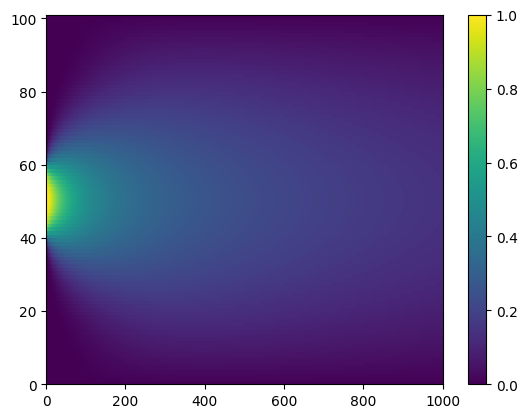
\includegraphics[scale=0.45]{./img/result_dif.png}}
    %\caption{Resultado difusión para $\alpha$ = 1}
    %\label{result_dif}
    %\end{figure}

    \begin{figure}[H] 
      \label{ fig7} 
    \begin{minipage}[b]{0.5\linewidth}
        \centering
        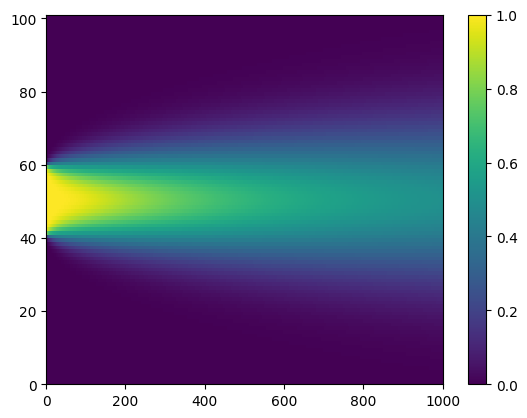
\includegraphics[width=.5\linewidth]{./img/alfa1.png}
      \caption{Instante $t$ = 0}\label{fig:awesome_image1} 
        \vspace{4ex}
      \end{minipage}%%
      \begin{minipage}[b]{0.5\linewidth}
          \centering
        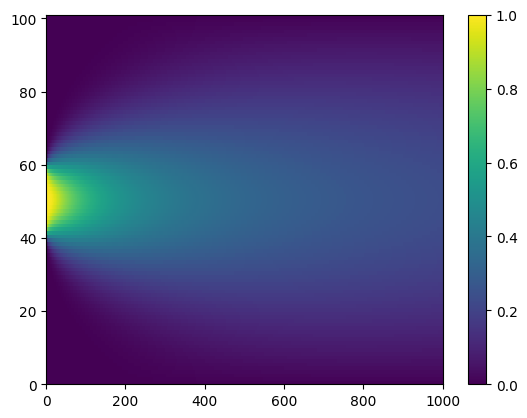
\includegraphics[width=.5\linewidth]{./img/alfa05.png} 
        \caption{Difusión $\alpha$ = 0.5} \label{dif0.5} 
        \vspace{4ex}
      \end{minipage} 
      \begin{minipage}[b]{0.5\linewidth}
        \centering
        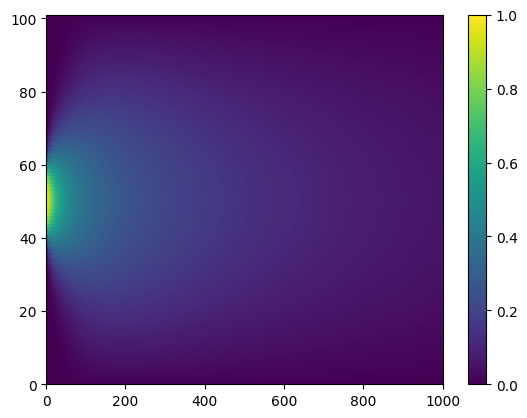
\includegraphics[width=.5\linewidth]{./img/alfa2.png}
      \caption{Difusion $\alpha$ = 2}\label{fig:awesome_image2}
        \vspace{4ex}
      \end{minipage}%% 
      \begin{minipage}[b]{0.5\linewidth}
        \centering
        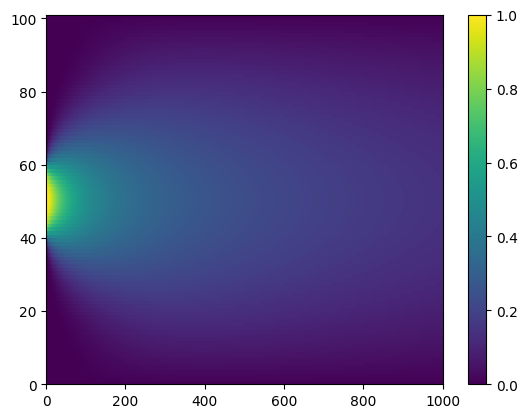
\includegraphics[width=.5\linewidth]{./img/result_dif.png}
      \caption{Difusión $\alpha$ = 1}\label{result_dif}
        \vspace{4ex}
      \end{minipage} 
    \end{figure}
\fi


%%%%%%%%%%%%%%%%%%%%%%%%%%%%%%

\iffalse
    \subsection{Resultado Difusión 2D}
    \label{difusion2D}
    \subsubsection{Ejercicio 7.1}

    \begin{figure}[H]
    \centerline{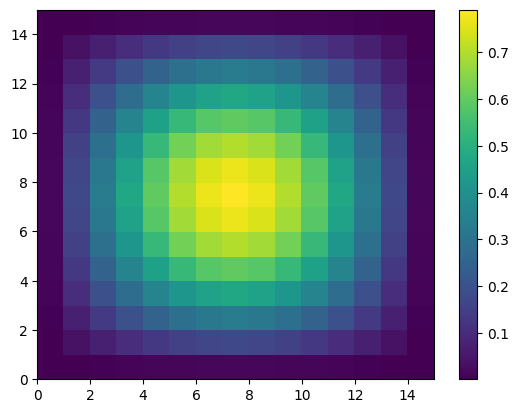
\includegraphics[scale=0.45]{./img/2Dcasoborde0.png}}
    \caption{Resultado simulación de difusión de calor en una placa 2D, condiciones de borde con temperatura 0}
    \label{result_dif}
    \end{figure}

    \subsubsection{Ejercicio 7.2}
    Realizando la comparación de los tiempos de cómputo para la resolución del sistema de ecuaciones de difusión de calor en 2D utilizando los dos métodos vistos anteriormente (eliminación gaussiana con y sin pivoteo) pudimos observar que, como era de esperar, el tiempo de cómputo aumenta de manera rápida a medida que el tamaño de la matriz crece. Esto se relaciona con el número de operaciones realizadas para resolver el sist. de ec. lineales ya que ésta crece aproximadamente de manera cúbica con el tamaño de la matriz.
    Para matrices pequeñas (hasta tamaño 10x10), el tiempo de cómputo es prácticamente el mismo por lo que sugiere que el pivote no añade un costo computacional significativo. Sin embargo, para matrices más grandes (12x12 en adelante), se empieza a notar una diferencia pues el pivoteo mejora la estabilidad numérica del sistema.

    \begin{figure}[H]
    \centerline{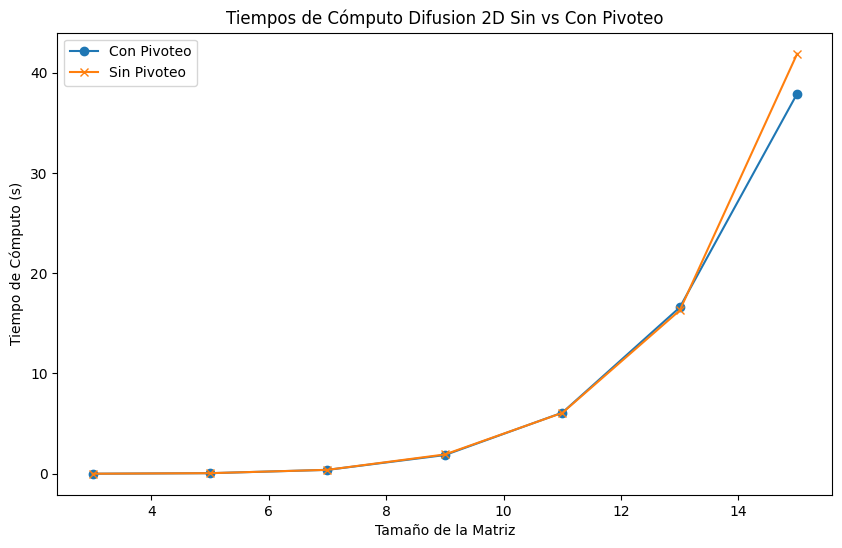
\includegraphics[scale=0.45]{./img/Dif2D_tiempos.png}}
    \caption{ Tiempos de cómputo para la resolución del sistema de ecuaciones de difusión de calor en 2D}
    \label{tiempos_dif2D}
    \end{figure}


    \subsubsection{Ejercicio 7.3}

    \begin{figure}[H] 
      \label{ fig7} 
      \begin{minipage}[b]{0.5\linewidth}
        \centering
        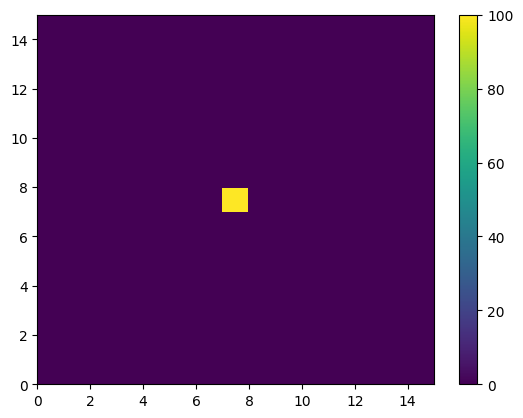
\includegraphics[width=.5\linewidth]{./img/instante_0.png}
      \caption{Instante $t$ = 0}\label{instante0} 
        \vspace{4ex}
      \end{minipage}%%
      \begin{minipage}[b]{0.5\linewidth}
         \centering
        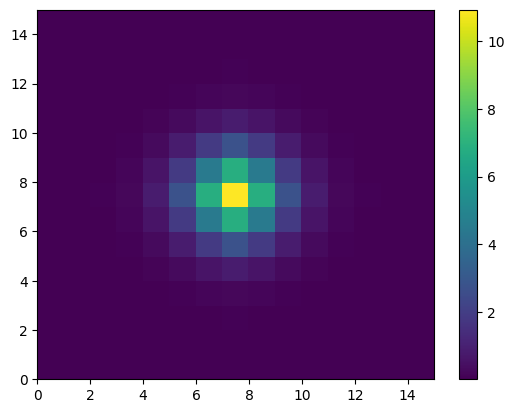
\includegraphics[width=.5\linewidth]{./img/instante_10.png} 
        \caption{Instante $t$ = 10} \label{instante10} 
        \vspace{4ex}
      \end{minipage} 
      \begin{minipage}[b]{0.5\linewidth}
        \centering
       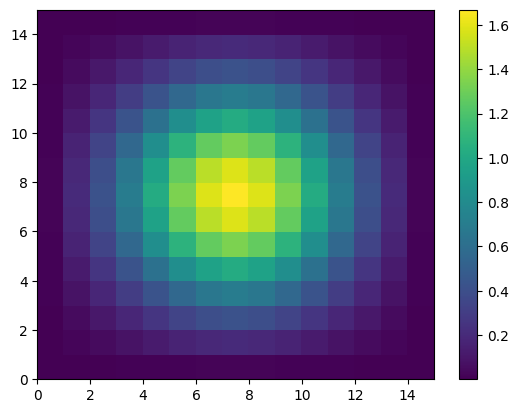
\includegraphics[width=.5\linewidth]{./img/instante_50.png}
      \caption{Instante $t$ = 50}\label{instante50}
        \vspace{4ex}
      \end{minipage}%% 
      \begin{minipage}[b]{0.5\linewidth}
       \centering
       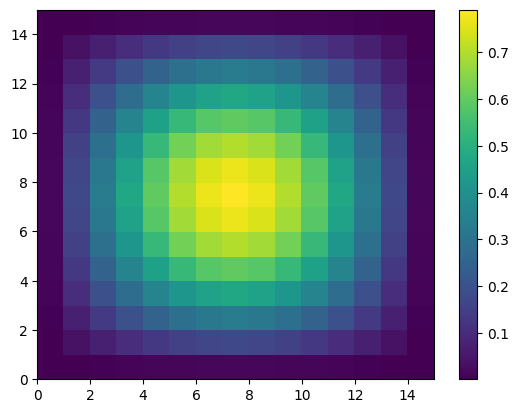
\includegraphics[width=.5\linewidth]{./img/instante_100.png}
      \caption{Instante $t$ = 100}\label{instante100}
        \vspace{4ex}
      \end{minipage} 
    \end{figure}


    \subsubsection{Ejercicio 7.4}
    Dado que los bordes tienen una temperatura fija de 0, el calor tenderá a disiparse hacia estos, lo que limitará su propagación.
    Podemos observar que en el instante t=10, el calor ya comenzó a propagarse significativamente desde el centro, pero todavía no ha llegado a los bordes de la placa, lo que es esperable porque aún estamos en un tiempo relativamente temprano en la simulación. A su vez, la distribución suave de la temperatura en los alrededores de la fuente central sugiere que el método implícito utilizado está funcionando bien, ya que evita oscilaciones o comportamientos inestables.
\fi


 \subsection{Cálculo de la inversa para una matriz}

 Como mencionamos en la sección \ref{opcionales}, el objetivo es calcular la matriz inversa de una matriz A utilizando el método de eliminación gaussiana (EG) con una matriz aumentada. Para ello se implemento la función \textit{invertir\_sistema} (algoritmo [\ref{alg:inversa}]), que sigue la idea del algoritmo contada en esa sección, cuyo pseudocódigo se puede ver a continuación.
 
\begin{algorithm}[H]
\caption{Inversa para una matriz dada}
\begin{algorithmic}
\State \textbf{EG}(\textbf{in} A : matrix) $\to \textbf{A\_inv}$
 
 \State $n \gets A.shape[0]$
 \State $I \gets matriz\_identidad$
 \State $new\_A \gets eg(A,I)$
 \State $base\_matrix \gets new\_A[0:,:n]$
 \For{$i \gets n$ to $2*n$}
        \State  b $\gets$ new\_A.(1,n)
        \State x $\gets$ resolver$\_$sistema(base$\_$matrix,b)
        \State A$\_$inv[0:,i-n] $\gets$ x
 \EndFor
 \State \textbf{return} $A\_inv$

\end{algorithmic}
\label{alg:inversa}
\end{algorithm}

Para resolver el problema utilizamos las funciones vistas en la secciones anteriores donde presentamos la eliminaci´ón gaussiana [\ref{sec:gaussiana}]. En la sección \ref{sec:inversa}, mostramos un ejemplo de su aplicación.
